\section{Intelligence as a Service}

\paragraph{} Il est important en premier lieu de comprendre comment est né le terme d'intelligence
artificielle et ce qu'il implique techniquement. L'IA est un domaine de l'informatique et se définit
comme l'étude des \emph{agents intelligents} : c'est-à-dire tout appareil en mesure de perçevoir son
environnement, et de prendre les actions en conséquence afin de maximiser ses chances de succès pour
le même objectif donné. \cite{AI0} Elle s'applique également aux fonctions cognitives qui
imitent l'humain, à l'exemple de \emph{l'apprentissage} ou de la \emph{résolution de problèmes}.

\paragraph{} Néanmoins, l'intelligence artificielle n'a pas toujours eu le même sens, ni comporté
tous les domaines présents aujourd'hui. Pour certains, elle désignerait uniquement ce qui n'a
pas encore été réalisé, comme la création d'une machine dotée d'une intelligence humaine et autonome.
On peut comprendre en ce sens que l'IA s'attache à essayer de conçevoir et de comprendre des faits
dans des domaines vastes et en perpétuelle évolution. Nous verrons par la suite que, même si
l'utilisation d'intelligences s'est \emph{démultipliée} de manière \emph{exponentielle} ces vingt
à soixante dernières années, le terme est encore utilisé parfois à tort ou de manière imprécise 
pour désigner des concepts mal compris. Cela s'explique notamment par l'utilisation abusive du terme 
par les médias, qui en font \emph{un buzzword}, et \emph{désinforment parfois} l'auditeur.
Par ailleurs, nous avons vu que la littérature et la science-fiction en particulier envisagent des
scénarii qui ne se révèlent pas nécessairement exacts. 

\paragraph{Objet d'étude} Les domaines d'études usuels de la recherche en intelligence artificielle sont le
\emph{raisonnement}, la \emph{perception}, l'\emph{apprentissage}, la \emph{connaissance}, la
\emph{prévision}, le \emph{traitement du langage naturel} (ou TLN, Natural Language Processing en anglais),
et en robotique l'habileté de \emph{se déplacer}, ou encore de \emph{déplacer} ou \emph{manipuler} des
objets. Son application nécessite l'utilisation d'outils comme l'\emph{optimisation}, la \emph{théorie des graphes},
mais aussi des méthodes statistiques et des notions de probabilité. 

\paragraph{Turing, adaptabilité, approches symbolique et connexionniste}

\paragraph{} Historiquement, c'est au milieu des années 50 qu'apparaît le termne d'intelligence artificielle, que l'on
doit à John McCarthy, aussi connu pour être le \emph{père de l'intelligence artificielle}. \cite{AI2} C'est également
dans les mêmes années qu'Alan Turing réalise un essai bien connu, \emph{The Imitation Game} (ou jeu d'imitation), procédé
permettant de déterminer si une machine est intelligente ou non. Pour cela, dans sa dernière version, le test de turing
propose à un être humain, placé dans une salle, de discuter avec deux personnes : une réelle, une autre simulée par une
machine. Si le sujet n'arrive pas à reconnaître quelle personne est réelle dans plus de la moitié des cas, alors on
considère que la machine à passé le test de Turing. \cite{Turing0}

\paragraph{} Ce test subit, à l'instar du test de QI, de nombreuses critiques. Il ne s'applique pas, en effet, à toutes
les formes d'intelligence mais uniquement aux programmes destinés à la communication. De plus, un programme \guillemotleft
non intelligent\guillemotright, c'est-à-dire conçu pour ruser le test, peut très bien le faire à l'exemple d'ELIZA.
\cite{Language0} Il utilise pour cela des mots de phrases précédentes qu'il réutilise pour poser des questions. Ce logiciel
se retrouve aussi comme psychologue dans l'éditeur de texte Emacs. \cite{Therapy0} Il est également intéressant de constater
que les logiciels \emph{trop intelligents} ne fonctionnent pas : en ne faisant jamais de fautes et en pratiquant une grammaire
et des tournures parfaites, le sujet se doute rapidement que son interlocuteur n'est pas humain.

\paragraph{} L'intelligence artificielle est donc une recherche \emph{d'adaptabilité}. Elle cherche à mettre en place des
stratégies \emph{souples}, qui répondent \emph{au mieux dans la plupart des cas}. On peut, dans ce grand courant, découper
deux types d'approches en particulier :
\begin{itemize}
    \item Symbolique : l'environnement et les lois qui s'y appliquent sont décrites avec le plus de précision possible,
    et il attendu du programme de choisir la meilleure option. C'est le cas par exemple des systèmes experts ou des
    logiques floues. Cette approche nous intéresse moins que la seconde car elle demande que les systèmes soient \emph{
    explicites}, et s'adapte donc mal à des cas \emph{réels}.
    \item Connexionniste : seul est donné au logiciel le moyen d'évaluer si ce qu'il fait est bien ou non - on le laisse
    en effet trouver des solutions \emph{seul, par émergence}. Les réseaux de neurones font partie de cette catégorie.
\end{itemize}

\paragraph{Utilisation de l'IA dans différents domaines}

\paragraph{} L'intelligence artificielle, nous la connaissons souvent le mieux associée avec la science-fiction. On
la vit parfois dangereusement, comme l'ordinateur HAL 9000 de l'Odyssée de l'Espace de Stanley Kubrick \cite{Kubrick0},
qui se rebelle contre les astronautes du vaisseau qu'il dirige. Asimov lui établit le code des robots dans son oeuvre
Le Cycle des Robots. \emph{Asimov1} Et l'IA est effectivement utilisée dans le monde de \emph{la robotique} pour permettre aux
robots d'intéragir de manière \emph{plus souple avec les humains qu'ils doivent aider}. \cite{AI1} Les tâches de ces 
robots peuvent être simples comme laver mais également bien plus complexe lorsqu'il s'agit par exemple d'aider une
personne n'ayant plus toutes ses capacités - une personne âgée ou en situation de handicap. Le domaine \emph{militaire} utilise
d'ailleurs l'IA à travers notamment de la robotique, avec l'utilisation de drones, la création de soldats mécaniques,
mais aussi des robots qui permettraient de localiser et sauver des victimes de catastrophes naturelles.

\paragraph{} Un autre grand domaine d'application de l'intelligence artificielle est le \emph{jeu vidéo}. L'utilisation 
d'automates et de chemins prédéfinis, comme les ennemis dans Mario par exemple, ne suffisent pas à permettre la réalisation
de jeux \emph{réalistes} dans certains domaines. On attend par exemple, dans un jeu de rôle ou un jeu d'aventure, que les
personnages aient un comportement qui paraisse le plus cohérent possible. Même des jeux très simples en terme de contenu
comme PacMan possèdent une part d'IA : chaque fantôme à un objectif différent.

\paragraph{} Et si la robotique et le jeu vidéo semblent des domaines d'application évidents, l'IA s'applique également
à bien d'autres domaines. Dans le milieu \emph{bancaire}, elle permet de détecter des fraudes à la carte bancaire. En
\emph{médecine}, certaines machines peuvent proposer des diagnostics en fonction des symptômes du patient, et ce de
manière plus rapide et complète qu'un médecin, même si ce dernier reste \emph{indispensable pour la prise de décision}.
En \emph{informatique industrielle} l'IA est utilisée en logistique, pour optimiser les trajets des transporteurs ou 
encore le remplissage de ces derniers. Le rangement d'un entrepôt peut également être optimisé grâce à des algorithme d'IA.
Les composants fabriqués peuvent être rendus plus efficaces, moins chèrs, en modifiant leur forme, leur composition ou 
leur disposition. L'intelligence artificielle s'applique en fait à \emph{toute situation à entrées données qui peut
être optimisable}.

\paragraph{Métaheuristiques, optimums, applications}

\paragraph{} Ces problèmes d'optimisation sont très courants dans la vie de tous les jours, et sont pourtant
difficiles à résoudre par un ordinateur - et encore plus par un humain - car le nombre de solutions est en
général très grand. Nous allons ici présenter les différentes techniques pour les résoudre, qui consistent 
en la recherche d'optimums globaux. Ces techniques sont aussi appellées métaheuristiques, des mots grecs \emph{meta}
(au-delà) et \emph{heuriskein} (trouver). Même s'il n'y a pas de consensus sur la définition d'une heuristique, nous
nous alignons avec la définition de S. Le Digabel \cite{Metaheuristics0} :

\begin{itemize}
    \item Une heuristique est une technique de résolution spécialisée à un problème. Elle ne garantit pas la qualité de
    la solution obtenue
    \item Une métaheuristique est une heuristique générique qu’il faut adapter à chaque problème
\end{itemize}

\paragraph{} Les métaheuristiques sont donc des \emph{stratégies} qui permettent de \emph{guider} la recherche vers une
solution optimale. Elle peuvent consister et des recherches d'optimums locaux comme en des processus d'apprentissage complexes,
sont non-déterministes et en ces sens ne garantissent pas l'optimalité.

\paragraph{} Un optimum, c'est un minimum ou un maximum. Lorsqu'il est local, cela signifie que c'est un optimum pour \emph{une
partie} de l'ensemble de définition de notre problème. Lorsqu'il est global, c'est alors un optimum pour \emph{tout l'ensemble
de définition} de notre fonction. On remarquera qu'il est possible d'avoir plusieurs optimums globaux. Nous nous interesserons 
uniquement aux minimisations, maximiser $f(x)$ consistant finalement à minimiser $-f(x)$.

\begin{figure}[h]
    \centering
    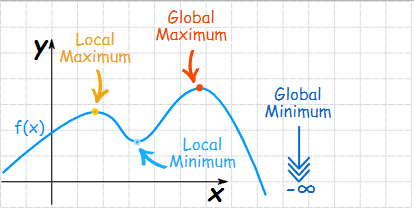
\includegraphics[width=250px]{chapters/03/images/optimums.png}
    \caption{\label{optimums} \emph{Local and global optimums}, \cite{Optimums0}}
\end{figure}

\paragraph{} Pour des fonctions simples, il est possible d'étudier ces dernières afin de trouver un minimum global.
C'est le cas pour des fonctions comme $f(x) = 2 + 1/x$ avec $x \in [1, 3]$ qui à un minimum en 3 où elle vaut $7/3$.
Cependant, dans la réalité, ces fonctions sont beaucoup trop complexes - en taille, en paramètres, en constructions
mathématiques - et nous avons alors recours aux \emph{métaheuristiques} et à la \emph{recherche exhaustive} afin
de trouver des solutions satisfaisantes. Il existe plusieurs métaheuristiques : \emph{algorithmes gloutons, descente
de gradient, recherche tabou, recuit simulé, par essaims particulaires}.. leur implémentation commentée est laissée
en annexe au lecteur curieux, aussi nous attarderons-nous ici sur les domaines d'application.

\paragraph{} Ces algorithmes sont régulièrement utilisés car ils interviennent lorsqu'il n'y a pas de moyen pour 
calculer un optimum de manière mathématique ou lorsque cela prendrait trop de temps. On espère alors obtenir un
résultat \emph{au plus proche} de la réalité. On les retrouve :
\begin{itemize}
    \item En \emph{électronique}, pour améliorer le design de cartes imprimées en minimisant le nombre de fils et 
    en minimisant la place requise par les différents composants.
    \item En \emph{finance}, où elles permettent d'optimiser un porte-feuille d'actions en cherchant à \emph{limiter
    les risques} ou en \emph{maximisant} les gains pour une somme donnée.
    \item En \emph{logistique}, dans des problèmes \emph{d'ordonnancement} comme par exemple créer les horaires pour
    des trains, bus ou avions. On va chercher par exemple à garder le moins possible les véhicules sur place (en gare, 
    aéroport).
    \item En \emph{conception}, pour trouver facilement les formes ou matériaux adéquats, ainsi qu'en \emph{construction}
    pour améliorer les formes des structures porteuses.
    \item Dans le domaine \emph{militaire}, principalement comme aide à l'homme afin \emph{de minimiser l'erreur
    humaine}. 
\end{itemize}

\paragraph{} Les applications de ces métaheuristiques sont donc \emph{diverses et variées}, grâce au caractère \emph{
adaptable} de ces dernières et à leur \emph{faible coût de mise en pratique}. Néanmoins, elle fournissent une
solution \emph{absolue}, et sont donc moins efficaces que d'autres catégories d'algorithmes lorsqu'il s'agit de traiter
de problèmes \emph{particuliers, spécialisés}. La recherche de chemins en est un bon exemple. 

\paragraph{Recherche de chemins, Théorie des graphes}

\paragraph{} De nombreux domaines font face à la recherche de chemins, dont le plus connu est certainement aujourd'hui
celui des GPS. Le champ est en fait bien plus vaste, car tous les problèmes associés peuvent être représentés sous
forme de \emph{graphes}, dont nous avons vu la forme naturelle précédemment (voir \ref{natural_networks}). Et nombreux
sont les problèmes pouvant être représentés sous la forme d'un graphe, à l'exemple de l'enchainement des mouvements pour
gagner au jeu d'echecs ou au jeu de go.

\paragraph{} Un graphe est \guillemotleft Un ensemble de \emph{noeuds} ou \emph{sommets} liés par des \emph{arcs}\guillemotright.
\cite{AI1} L'exemple suivant est un graphe simple comportant 18 sommets et 17 arcs. On parle de \emph{circuit} lorsqu'on
peut partir d'un noeud et y revenir en ne passant pas deux fois par le même arc. L'ordre d'un graphe correspond au nombre
de sommets qu'il contient, et enfin deux n\oe{}uds sont dits \emph{adjacents} s'il existe un arc permettant d'aller de
l'un à l'autre.

\begin{figure}[h]
    \centering
    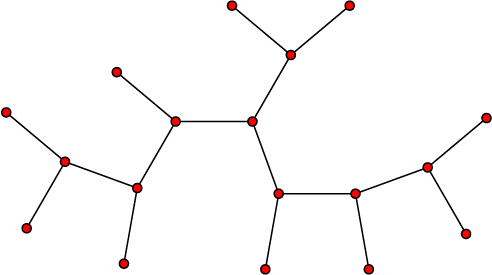
\includegraphics[width=250px]{chapters/03/images/simple_graph.png}
    \caption{\label{graph}\emph{Simple graph}, \cite{GraphTheory0}}
\end{figure}

\paragraph{} Il existe plusieurs manières de représenter un graphe. La première est \emph{graphique}, comme dans 
l'exemple ci-dessus. Ici, l'ordre et le placement des n\oe{}uds importent peu, mais on va toujours chercher à placer
l'ensemble de sorte à rendre le graphe \emph{le plus lisible}, en décroisant les arcs par exemple. Mais cette représentation
n'étant pas très pratique pour l'utilisation d'algorithmes, on préfèrera alors utiliser une \emph{matrice d'adjacence}.
Pour cela, il suffit de représenter, \emph{dans un tableau à deux dimensions}, l'ensemble des \emph{adjacences entre les
sommets} du graphe. Si, comme dans le cas précédent, le graphe ne possède pas \emph{de poids}, on peut alors numéroter
notre matrice par un système binaire : 0 quand il n'y a pas de connexion et 1 quand il y en a une. Si, comme dans le cas
suivant, notre graphe possède des poids, c'est à dire que le chemin \emph{entre deux n\oe{}uds possède une valeur}, on
utilisera le signe $\infty$ lorsque deux n\oe{}uds ne sont pas reliés par un arc, et 0 pour le coût entre un n\oe{}ud et
lui-même.

\begin{figure}[h]
    \centering
    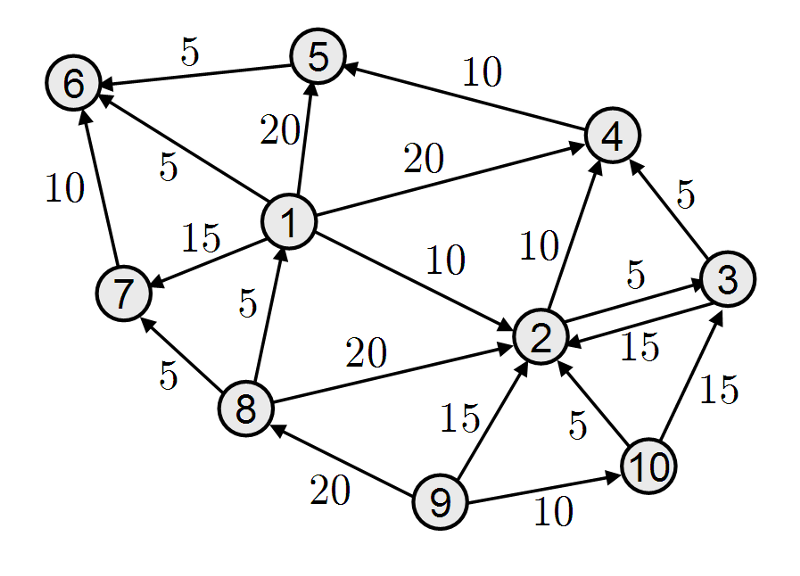
\includegraphics[width=250px]{chapters/03/images/weighted_graph.png}
    \caption{\label{weighted_graph}\emph{Graph with weights}, \cite{GraphTheory1}}
\end{figure}

\paragraph{} Afin de travailler sur des graphes, nous pouvons utiliser deux catégories d'algorithmes : ceux dit \emph{naïfs},
et ceux dits \emph{intelligents}. L'ensemble des algorithmes présentés le seront sur leur démarche. Le code associé est
disponible en annexe pour le lecteur qui souhaiterait en connaître une application.

\paragraph{Algorithmes naïfs} Ces derniers sont appelés ainsi car ils n'utilisent pas de connaissances sur le problème
pour agir. Ils vont donc, dans le pire des cas, tester tous les chemins possibles pour vérifier l'existence d'un chemin
entre deux n\oe{}uds. De plus, ils ne garantissent pas que le chemin trouvé est bien le plus court ; ils sont 
néanmoins \emph{faciles à implémenter}. Deux exemples connus de ces algorithmes sont les suivants :
\begin{itemize}
    \item Le \emph{parcours en profondeur}. C'est celui qu'on utilise \emph{naturellement} dans un labyrinthe, il consiste
    à avancer le plus possible jusqu'à être coincé, puis revenir sur la dernière intersection et tester un nouveau chemin.
    Cet approche repose en immense partie sur \emph{la stratégie de parcours} que de l'on décide d'appliquer. Dans un labyrinthe
    par exemple, il est possible que choisir l'ordre d'importance (gauche, droite, milieu) nous aurait fait parvenir plus vite
    à la sortie que (droite, milieu, gauche). Cet algorithme n'est donc pas souvent efficace, de plus il faut qu'il teste
    en moyenne un grand nombre de possibilités pour trouver un chemin.
    \item Le \emph{parcours en largeur}, que l'on peut assimilier au trajet que fait \emph{la police pour retrouver un
    coupable}. On part du derner point où il à été vu et on s'en éloigne en cercles concentriques. Ainsi, il n'est plus
    question d'ordre, mais cet algorithme n'est \emph{pas du tout efficace}. Néanmoins, si tous les arcs \emph{ont le
    même poids}, nous serons assurés de \emph{trouver le chemin le plus court}.
\end{itemize}

\paragraph{Algorithmes intelligents} Etant donné que les parcours présentés ne permettent pas de trouver le chemin
le plus court, ni de le faire dans un temps acceptable, il nous faut utiliser d'autres algorithmes. Nous avons pour
cela plusieurs options dont nous allons présenter les trois les plus connues : algorithme de Bellman-Ford, de Dijkstra,
et A* (ou A étoile).

\paragraph{} L'algorithme de Bellman-Ford nous garantit de trouver le chemin le plus court s'il en existe un. Ce n'est pas
le plus optimisé mais celui qui fonctionne dans le plus de cas, car il accepte en effet des valeurs \emph{négatives} pour les
arcs. De plus, s'il y a un circuit dont le \emph{poids total est négatif}, il peut le repérer et statuer qu'il n'existe alors
pas de chemin le plus court. Il utilise la matrice des longueurs et est itératif. Après avoir initialisé à $+\infty$ la 
longueur minimale de chaque n\oe{}ud, il parcourt chaque arc et met à jour les distances au n\oe{}ud courant si elles sont
plus faibles. Il passe ensuite au n\oe{}ud suivant avec le poids le plus faible et réitère son procédé jusqu'à ce qu'il ait
obtenu le chemin \emph{le plus court}.

\paragraph{} L'algorithme de Dijkstra, certainement le plus connu des algorithmes de \emph{pathfinding}, est une amélioration
de l'algorithme de Bellman-Ford, qui ne fonctionne que si toutes les distances sont positives. On remarquera que c'est généralement
le cas dans les problèmes réels. Il se démarque en choisissant plus intelligemment l'ordre d'application des distances. En effet,
au lieu de s'appliquer sur les arcs, il s'applique \emph{sur les noeuds}, et il ne revient jamais en arrière. De cette manière,
chaque arc ne sera appliqué \emph{qu'une fois}. L'application des distances n\oe{}ud par n\oe{}ud permet une \emph{
optimisation} en terme de calculs et donc en terme \emph{de temps}.

\paragraph{} Enfin, l'algorithme A* ne teste pas tous les chemins et ne peut pas assurer que le chemin trouvé est le
plus court. Dans des cas comme le labyrinthe il sera très peu ou pas efficace, alors que c'est sur des espaces ouverts,
avec peu d'obstacles qu'il sera très performant. Cet algorithme utilise des informations sur la localisation de son
objectif afin de choisir la direction. En effet, à la manière d'un homme qui se repère dans une ville, A* se fonde sur le
fait que la distance la plus courte \emph{est généralement la ligne droite}. Plus son approximation de la distance 
restante entre chaque n\oe{}ud et la sortie est précise, et plus l'algorithme sera efficace. Dans son fonctionnement, A*
est semblable aux algorithmes précédents à l'exception importante qu'il visite toujours \emph{le n\oe{}ud le plus
prometteur} en suivant.

\paragraph{Domaines d'application}

\paragraph{} Tous ces algorithmes sont utilisés dans de nombreux domaines. Un premier exemple évident
est \emph{la recherche d'itinéraires}. Tous les logiciels qui permettent de se déplacer, quelque soit le moyen,
tous les GPS utilisent des algorithmes de \emph{pathfinding}. Etant donné les modèles complexes sur lesquels
ils s'appuient parfois (comme par exemple \emph{Google Maps}), ces algorithmes doivent être \emph{bien optimisés},
et privilégier \emph{les grands axes} quand ils le peuvent. Il est intéressant de constater que le détail de tels
algorithmes n'est pas communiqué - nous defendons en effet la publication ouverte de tous les logiciels permettant de près
ou de loin d'avoir des activités proches du \emph{tracking}.

\paragraph{} Le \emph{pathfinding} est également très utilisé dans les \emph{jeux vidéos}, en particulier l'algorithme A*
qui est très efficace comme nous l'avons vu lorsqu'il s'agit de trouver des chemins dans des espaces \emph{ouverts}, ou
avec \emph{peu d'obstacles}. Son efficacité est particulièrement appréciée dans le milieu du jeu vidéo qui est 
un environnement riche en contraintes d'optimisation. En \emph{robotique}, la recherche de chemins permet à un robot,
dans une \emph{situation réelle}, de trouver le meilleur chemin pour aller à un endroit, et ce \emph{en prenant compte des
modifications en temps réel de l'environnement}.

\paragraph{} Dans \emph{les réseaux}, des algorithmes de \emph{pathfinding} sont utilisés pour le \emph{routage}. Internet
en est un excellent exemple, où le protocole RIP (pour \emph{Routing Information Protocol}) utilise ainsi Bellman-Ford, en
envoyant toutes les 30 secondes les nouvelles routes. \cite{AI1} Aussi le protocole OSPF, qui à été inventé en premier lieu
pour remplacer RIP, fonctionne avec l'algorithme de Dijkstra, qui est comme nous l'avons vu une amélioration de l'algorithme
de Bellman-Ford. Enfin en \emph{théorie des jeux}, où l'espace de possibilités est en général \emph{bien trop vaste}, ils
permettent d'approcher des positions gagnantes, ou du moins \emph{plus intéressantes que celle de départ}.

\paragraph{} ------------------------------------

\paragraph{Smartphones et IA}

\paragraph{} La révolution du smartphone. La démocratisation de l'IA dans le smartphone.
Quel avenir pour l'IA ?

\paragraph{Objectif} L'objectif est d'ajouter ici des traitements de données automatisés au section
du Réseau.

